\documentclass[10pt,conference]{IEEEtran}
% \IEEEoverridecommandlockouts
% The preceding line is only needed to identify funding in the first footnote. If that is unneeded, please comment it out.
\usepackage{cite}
\usepackage{amsmath,amssymb,amsfonts}
\usepackage{algorithmic}
\usepackage{graphicx}
\usepackage{textcomp}
\usepackage{xcolor}

\usepackage{listings}
\usepackage{xcolor}



\newcommand\question[1]{{\color{violet}#1}}
\newcommand\todo[1]{{\color{red}#1}}


\definecolor{codegreen}{rgb}{0,0.6,0}
\definecolor{codegray}{rgb}{0.5,0.5,0.5}
\definecolor{codepurple}{rgb}{0.58,0,0.82}
\definecolor{backcolour}{rgb}{0.97,0.97,0.97}

\lstdefinestyle{mystyle}{
    backgroundcolor=\color{backcolour},
    commentstyle=\color{codegreen},
    keywordstyle=\color{magenta},
    numberstyle=\tiny\color{codegray},
    stringstyle=\color{codepurple},
    basicstyle=\ttfamily\footnotesize,
    breakatwhitespace=false,
    breaklines=true,
    captionpos=b,
    keepspaces=true,
    numbers=left,
    numbersep=5pt,
    showspaces=false,
    showstringspaces=false,
    showtabs=false,
    tabsize=2
}

\lstset{
%   basicstyle=\ttfamily,
  mathescape
}



\usepackage{minted}
\usepackage{hyperref}


% \bibliographystyle{ieeetr}

\def\BibTeX{{\rm B\kern-.05em{\sc i\kern-.025em b}\kern-.08em
    T\kern-.1667em\lower.7ex\hbox{E}\kern-.125emX}}
\begin{document}

\title{Hardware and Software Co-Design for Sparse Linear Algebra Operations Acceleration 
}

\author{\IEEEauthorblockN{Aleksey Tyurin}
\IEEEauthorblockA{\textit{Saint Petersburg State University} \\
Saint Petersburg, Russia \\
alekseytyurinspb@gmail.com}
\and
\IEEEauthorblockN{Daniil Berezun}
\IEEEauthorblockA{\textit{Saint Petersburg State University} \\
\textit{JetBrains Research}\\
Saint Petersburg, Russia \\
d.berezun@2009.spbu.ru}
\and
\IEEEauthorblockN{Semyon Grigorev}
\IEEEauthorblockA{\textit{Saint Petersburg State University} \\
\textit{JetBrains Research}\\
Saint Petersburg, Russia \\
s.v.grigoriev@spbu.ru}
}


\maketitle

%% Abstract
%% Note: \begin{abstract}...\end{abstract} environment must come
%% before \maketitle command
\begin{abstract}

In the era of big data, computations are expected to be faster and less power-consuming in order to become more effective and affordable. 
And when modern CPUs and GPUs appear to be underutilized due to being too general-purposed for some problems, application-specific hardware accelerators are able to provide the needed performance.
This is particularly the case for sparse linear algebra problems for which a number of hardware accelerators have been designed.
In this work, we elaborate on the optimizations that are missed out in present accelerators due to the lacking of a software part of an accelerator. 
We propose a co-design approach that could potentially exploit such optimizations and still have decent hardware acceleration.
% Sparse linear algebra is a great framework for building algorithms in a uniform and optimization-amenable way.
% However, CPUs and GPUs currently running such algorithms are underutilized due to being too general-purposed for problems that include sparsity.
% Thus, an application-specific integrated circuit could speed sparse computations up, following the example of \textit{Google TPU's}.
% It is worth noting that such a circuit needs to be not self-contained to allow some expected optimizations to be made by a compiler or a framework itself.
% Finally, the optimizations should be easily definable in the language and as automated as possible, thus a careful simultaneous design of hardware and software is needed.
% The proposal describes the bottlenecks inherent to present sparse linear algebra framework implementations, summarizes the expected optimizations, and proposes a co-design approach to designing a highly-optimized sparse linear algebra framework.
% \textit{This is a work in progress and not yet present the final result}.


\end{abstract}


\section*{Introduction}
Linear algebra is a great instrument for solving a wide variety of problems utilizing matrices and vectors for data representation and analysis with the help of highly optimized routines.
And whilst the matrices involved in a vast diversity of modern applications, e.g., recommender systems~\cite{gupta2020architectural,amazon} and graph analysis~\cite{graph1,graph2}, consist of a large number of elements, the major part of them are zeros.
Such a high sparsity incurs both computational and storage inefficiencies, requiring unnecessarily large storage, occupied by zero elements, and a large number of operations on zeroes, where the result is obviously known beforehand.
The traditional approach to address these inefficiencies is to compress the matrix and store only the non-zero elements. 
Thus, the effect of matrices tending to be sparse in many applications makes the techniques of matrix compressed representation and sparse linear algebra to be the effective way of tackling problems in areas including but not limited to graph analysis~\cite{GAILLA}, computational biology~\cite{compBio}, and machine learning~\cite{Kepner_2017}.



Sparse linear algebra defines primitives for expressing algorithms for the mentioned areas in a uniform way in terms of sparse matrix and vector operations parameterized by a semiring.
Such uniform representation allows tunning the whole bunch of expressible algorithms through optimizing the primitives solely.
One of the most used primitive is a sparse matrix-sparse matrix multiplication (spMspM) operation. 
It has finely-tuned implementations for both CPU and GPU, which, however, are proven to be underutilized due to the memory-bound nature of sparse computations induced by compressed representation~\cite{Florida,leskovec2016snap,Song_2016,zhang2020sparch}.
Further, the pipeline of spMspM is patchy, which makes some of the computational units to be idle from time to time as it could be seen in figure~\ref{fig:sm_util}, while the peak FLOPS is less than 1\% of maximum available\footnote{\url{https://hanlab.mit.edu/projects/sparch/} (Accessed 09.02.2021)}. 


\begin{figure}[t]
  \centering
  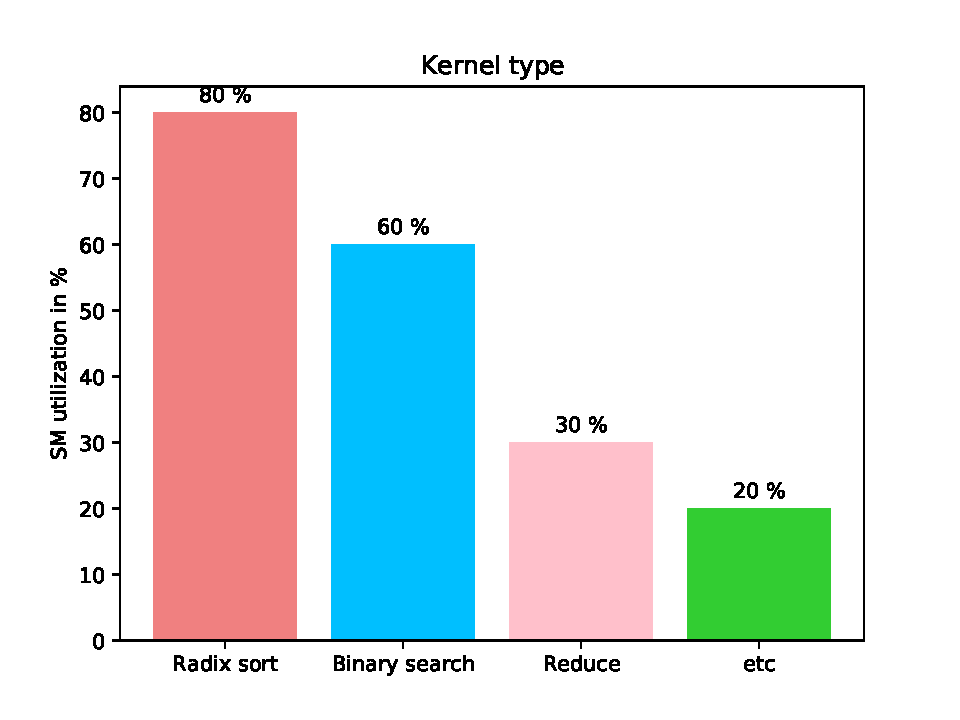
\includegraphics[width=\linewidth]{figs/SM_performance.pdf}
  \caption[Caption for LOF]{GPU's SM utilization for spMspM pipeline from cuSPARSE\footnotemark}
  \label{fig:sm_util}
\end{figure}

\footnotetext{\url{https://developer.nvidia.com/cusparse} (Accessed 09.02.2021)}

\begin{listing}
  \caption{Sequence of sparse operations example}
\label{listing:1}

\begin{minted}[]{haskell}
  -- A,B,C,D are sparse matrices
  -- M is a mask
  D<M> = A eWiseAdd B eWiseMult C
\end{minted}

\end{listing}

This makes the typical CPUs and GPUs not well-suited hardware for sparse computations and gives a rise to specialized hardware accelerators, which are primarily concerned with spMspM.
However, for a sparse framework to be useful, it should incorporate not only spMspM, but also other sparse operations like in listing~\ref{listing:1}, where masking, which filters the matrix elements, and element-wise operations (possibly parameterized by a semiring) needed for, e.g., PageRank and bread-first search (BFS) algorithms~\cite{yang2020graphblast},  are presented.
Such operations are assembled in \emph{GraphBLAS}~\cite{buluc2017graphblas} specification and could be used as building blocks to construct many algorithms~\cite{compBio,Kepner_2017,GAILLA}.
When such operations are chained explicitly or implicitly, via a loop body, certain optimizations could be applied, like the one that eliminates intermediate matrices in sequence from listing~\ref{listing:1}.
Unfortunately, some of such optimizations (e.g., the one mentioned) are only expressible at a software level, i.e., in a programming language, hence modern spMspM accelerators could be impractical for accelerating the whole program representing a sparse linear algebra-based algorithm like PageRank or BFS, due to the lack of a software part and to a too narrow hardware specialization.

Thus a co-design of dedicated hardware and software components, i.e., domain-specific processor (DSP) and a corresponding domain-specific language (DSL), could provide a system that is not more efficient for spMspM than present hardware accelerators, but appear to be more effective in terms of speed and power consumption for holistic pieces of program, i.e., for chained operations, than current CPUs and GPUs implementations.
The ongoing work is devoted to the design of respective DSL, DSP, and an optimizing compiler, and this work, in particular, gives a brief overview of the field, discusses the ideas and challenges behind the design. 


\section{Problem Statement}
Since sparse linear algebra applications are mostly concerned with graph problems, some of the optimizations are graph-specific~\cite{yang2020graphblast,graphIt}, e.g., direction optimization.
However, in memory-bound applications optimizations that minimize data transfer are essential. 
For example, \emph{kernel fusion} is a wide-addressed optimization that fuses multiple operations into one, avoiding intermediate memory accesses, utilizing, e.g., registers to pass the data between the operations.
In the case of sparse linear algebra frameworks kernel fusion is not yet widely implemented, but most often related to fusing chained operations like
% \begin{minted}[escapeinside=//]{haskell}
%   D<M> = A eWiseAdd B eWiseMult C
% \end{minted}
from listing~\ref{listing:1} to avoid intermediate matrices construction and reduce memory accesses with masking~\cite{yang2020graphblast}.

The problem of intermediate data structures is common for functional programming
and there have been developed a number of 
optimization techniques that try to reduce intermediate 
data structures or computations, namely partial evaluation~\cite{jones}, deforestation~\cite{WADLER1990231}, supercompilation~\cite{supercompilation}, and distillation~\cite{distillation}.

These fusion family optimizations are implementation-dependent, meaning that the optimizer should have an access to the source code, which is impossible when the function is implemented solely in hardware, hence a software part is inevitable in the design of a system that tries to put together fusion and hardware.
Thus, present hardware accelerators are not general enough to implement and accelerate a whole sparse linear algebra-based program, e.g., do not provide arbitrary semiring support, and lack a software part hence leaving out essential optimizations.
General-purpose devices such as GPUs are hard to perform some optimizations, e.g., fusion requires two GPU kernels to have the same memory access pattern and partial evaluation could induce some thread divergence due to SIMD nature of a GPU. 
Further, present systems that support fusion are domain-specific\footnote{\url{https://www.tensorflow.org/xla} (Accessed 09.02.2021)}, or perform the optimization on top of data structures that may not be suitable for sparse operations (mainly for effective compressed representation), e.g., streams and lists~\cite{StreamFusion,StreamFusion2}, while array-based fusion systems do not perform fusion with index arithmetic~\cite{Futhark}.
Finally, some data needed for optimizations~\cite{jones} is only available in runtime, thus there should be support for JIT optimizations.
The design of the proposed hardware-software system should take these challenges into consideration. 
Next, we discuss hardware accelerators from adjacent areas and elaborate on the software optimization we want to exploit.

\section{Graph Processors}

Sparse linear algebra is often concerned with graph problems, and since
graph processing is mature enough to be considered as a distinct computation paradigm, there have been emerged a number of graph processors~\cite{GraphProcessors} to mitigate the issues of graph processing on general-purpose processors.
Presently, many proposed accelerator models are not generic, in the sense, they are optimized for specific
classes of graph algorithms and lack scalability. Further, sparse linear algebra makes graph computations more amenable to effective parallelization, ease scalability, and even spreads beyond graph computations~\cite{compBio}. 

There is definitely a research interest in the design of sparse linear algebra-based instruction set processor~\cite{Song_2016}, but the design in~\cite{Song_2016} at the moment provides only spMspM operation and does not mention a software part as one of its key components.
Other sparse linear algebra accelerators~\cite{CPU-FPGA,OuterSpace,zhang2020sparch} are applicable only to certain operations like spMspM.
Notably, in~\cite{smash} the way of compressed representation of a sparse matrix is identified as the main bottleneck and an approach for hardware acceleration for compressed representation indexing is proposed, which is able to employ existing optimizations and could be integrated into existing software frameworks.
Hence, the underlying hardware is better to support the indexing needed by a compressed representation of choice to be effective.
However, we believe that to fully leverage fusion the indexing should be transparent, i.e., constructive, in the software, which is not the case in~\cite{smash}.

\section{Supercompilation}
Supercompilation~\cite{supercompilation} could be thought of as a combination of many optimizations designed to reduce the number of data structures and the number of computations in general for functional programming languages~\cite{distillation,WADLER1990231,jones}.
In particular, partial evaluation~\cite{jones} stands for precomputing the parts of a program that depend on statically known data. Interestingly, some data may become static in runtime, e.g., it could remain fixed between different iterations of a loop, thus it may be profitable to perform such optimization even in runtime.
Despite such optimizations are common in the world of functional programming, they are hard to perform in the case of imperative languages widely used in high performance computing.
However, a fully working supercompiler at the moment is developed only for a small functional language~\cite{hosc}, since being too hard to implement for a rich language like Haksell. But we believe that such a small language is enough to provide a DSL for sparse linear algebra with the help of syntactic sugar and custom fusion rules.
Also, such optimization may produce a burden of \texttt{case} statements, which slow down the hardware that exploits SIMD model, hence they could not be executed in parallel.
Finally, fusion performed, e.g., by a supercompiler heavily depends on the compressed representation, i.e. presently quadtree representation seems to fit more for fusion than, e.g., coordinate format. 
Some operations could not be fused in principle, e.g. sorting, but the need for some of such operations could be induced by the compressed representation once again, e.g., quadtree representation does not require sorting, so it is reasonable to implement non-fusable operations in hardware.


\section{Functional Language Processors}
The functional DSL is not of much use until effectively compiled for DSP, therefore it is tempting to utilize state-of-the-art processors developed to  
add hardware support for functional programming~\cite{ACqua,Reduceron,PILGRIM}. Where \cite{ACqua} leverages the parallelization of independent function calls and also
provides optimized support for lists and \texttt{map} operation specifically, which may not be the desired property due to the compressed representation of choice. The general-purpose nature of such processors could also hurt sparse operations performance due to non-specialized cache.
Further, they focus on hardware support for graph reduction via parallelization, specialized memory, and pipelining, thus even more parallelism could be extracted from a compressed representation with their help.

However, present functional processors could be too complex to integrate with, e.g., to add hardware support for indexing or another computation that cannot be optimized effectively in software. 
Instead, we plan to opt for a more flexible solution and want to leverage the approach of dataflow representation of functional programs with indirect memory accesses~\cite{funcHLS}, which then could be effectively represented in hardware in a highly parallel way. 
The approach currently generates application-specific RTL code, but we hope to adapt it for dataflow processor architecture, e.g., transport-triggered-architecture (TTA), in order to have a highly scalable and parallel processor with hardware support for a compressed representation, able to run functional programs and easily extensible with custom operations. 

% Thus, we need to explore the potential of different compressed representations in terms of hardware support and fusion. A prominent candidate is a quad-tree representation, which is more amenable to supercompilation (and hence to fusion), \todo{while a program after supercompilation basically represents a dataflow through pattern matching and semiring operations}.


\section{Research Questions and Roadmap}
We propose the co-design of a hardware/software system for sparse linear algebra acceleration to address the mention problems and challenges of optimizeability and expressibility.
We believe that a functional DSL, where an arbitrary semiring could be concisely and conveniently expressed, powered by a set of optimizers and compilable to some DSP with enough parallelism could be a good starting point.
The solution should include the simultaneous design of the following components.
\begin{itemize}
  \item Functional DSL to develop a library of sparse linear algebra operations, since 
  functional programming language is appear to be well-suitable for supercompilation and specialized hardware creation.
  The language should be minimized to simplify optimizations and compilation, but expressive enough to implement a sufficient subset of GraphpBLAS specification.
  \item Compiler from the functional DSL to the specialized hardware. 
  \item Supercompiler for the functional DSL. The supercompiler should be designed for multistage processing.
  For example, the first stage could be a compile-time fusion of functions, and the second stage could be a partial evaluation on some data. 
  This allows one to exploit dynamic data as static, and minimize overhead in running time. 
  \item Library of sparse linear algebra operations, i.e., GraphBLAS specification implementation, in the functional DSL.
  We should choose such representation of vectors and matrices, and such principles of code design that both allow software optimizations and efficient hardware design should be possible.  
  \item Special hardware, which should be general enough to execute all the code written in the functional DSL that utilizes the library of sparse linear algebra operations.  
\end{itemize}

Such a multicomponent solution with nontrivial connections between components requires deep analysis in a number of areas.
So, at the first stage, we plan to focus on the following questions.
\begin{enumerate}
  \item Is supercompilation suitable for required optimizations? For example, is it able to remove intermediate matrices creation in chained operations, like presented in listing~\ref{listing:1}.
  \item Can we generate program-specific hardware from the sparse linear algebra-based program written in a functional programming language such that it will be efficient in comparison with current solutions?
  \item Is supercompilation suitable in functional-program-to-hardware workflow? Does a supercompiled program compile to more efficient hardware than the original one?
  \item Does staged supercompilation allow to minimize partial evaluation time enough to apply partial evaluation in runtime? 
\end{enumerate}

As a first step, we plan to write a prototype comprising operations like multiplication, element-wise addition, Kronecker product, and masking in a minimalistic functional programming language (Haskell-core) and try to apply HOSC~\cite{hosc} to it with the focus on a more amenable to supercompilation quadtree compressed representation. 
It would allow us to estimate supercompilation effect in terms of expected optimizations like fusion, and time required for partial evaluation. 
Also, at this step, we should establish some principles of the library design that maximize supercompilation effect.

At the same time, we plan to evaluate functional language to hardware compiler~\cite{funcHLS} on the developed library to estimate the performance of the implemented operations and to compare basic and supercompiled versions.

As a result of this step, we expect to estimate applicability of functional programming language and related optimization techniques for the creation of high-performance sparse linear algebra-based solutions as well as the suitability of dataflow approach to DSP architecture. 
In the end, we should provide a solution for program-specific accelerators creation for sparse linear algebra-based subprograms. 

As far as the final goal is to create not a program-specific hardware accelerator, but a processor unit for high-performance sparse linear algebra-based computations, the second stage would be focused on the following strongly connected questions. 
\begin{enumerate}  
  \item Can we generalize ideas from functional languages to hardware compilation to create a specific processor unit for sparse linear algebra? In other words, is that possible to generalize the dataflow approach of compiling a functional program to RTL description to compiling a functional program to a dataflow processor?
  \item Can the designed language be efficiently compiled to the designed processor unit?
\end{enumerate}

As a result of this stage, we hope to create a specialized processor unit for sparse linear algebra and a compiler from the functional DSL to it.
We plan, that generalization will be based on the transformation of the program-specific dataflow diagram to TTA-like processor by reusing functional units with respective compiler development.


The final stage is the creation of SDK to integrate the DSL into an application. 
The SDK should provide tools for staged optimizations, communication with the special processor unit, and interoperability with general-purpose programming languages. 


%% Bibliography
\bibliographystyle{./IEEEtran}
\bibliography{bib}


%% Appendix
% \appendix
% \section{Appendix}

% Text of appendix \ldots


\end{document}